\documentclass[10pt,a4paper]{article}
\usepackage[margin=18mm]{geometry}
\usepackage[T1]{fontenc}
\usepackage{lmodern,microtype}
\usepackage{amsmath,amssymb,booktabs}
\usepackage{graphicx,xcolor}
\usepackage[numbers,sort&compress]{natbib}
\usepackage[hidelinks]{hyperref}
\usepackage{caption}
\captionsetup{font=small,labelfont=bf,skip=4pt}
\definecolor{ink}{HTML}{1F2933}
\setlength{\parskip}{4pt}
\setlength{\parindent}{0pt}
\setlength{\emergencystretch}{2em}
% Generated by scripts/cellbridge_numbers_v100.py. Do not edit by hand.
\newcommand{\Num}[1]{#1}
\newcommand{\NGseTrain}{11}
\newcommand{\NGseCal}{9}
\newcommand{\NGseTest}{10}
\newcommand{\NEmTrain}{64}
\newcommand{\NEmCal}{31}
\newcommand{\NEmTest}{29}
\newcommand{\MaeGseCbEone}{0.284}
\newcommand{\MaeGseCbEtwo}{0.322}
\newcommand{\MaeGseAbEone}{0.315}
\newcommand{\MaeGseAbEtwo}{0.359}
\newcommand{\MaeGseTvEone}{0.393}
\newcommand{\MaeGseTvEtwo}{0.395}
\newcommand{\MaeGseRoEone}{0.376}
\newcommand{\MaeGseRoEtwo}{0.461}
\newcommand{\MaeGseJtEone}{0.756}
\newcommand{\MaeGseJtEtwo}{0.722}
\newcommand{\MaeGseRnEone}{0.799}
\newcommand{\MaeGseRnEtwo}{0.755}
\newcommand{\MaeGseMnEone}{0.511}
\newcommand{\MaeGseMnEtwo}{0.643}
\newcommand{\MaeEmCbEone}{0.530}
\newcommand{\MaeEmCbEtwo}{0.471}
\newcommand{\MaeEmAbEone}{0.526}
\newcommand{\MaeEmAbEtwo}{0.472}
\newcommand{\MaeEmTvEone}{0.929}
\newcommand{\MaeEmTvEtwo}{0.844}
\newcommand{\MaeEmRoEone}{0.889}
\newcommand{\MaeEmRoEtwo}{0.815}
\newcommand{\MaeEmJtEone}{0.889}
\newcommand{\MaeEmJtEtwo}{0.824}
\newcommand{\MaeEmRnEone}{0.889}
\newcommand{\MaeEmRnEtwo}{0.824}
\newcommand{\MaeEmMnEone}{0.889}
\newcommand{\MaeEmMnEtwo}{0.824}
\newcommand{\GseHOneGain}{0.321}
\newcommand{\GseHOneLo}{0.238}
\newcommand{\GseHOneHi}{0.410}
\newcommand{\GseHOneP}{=0.002}
\newcommand{\GseHOneWins}{10}
\newcommand{\GseHOneN}{10}
\newcommand{\GseHOneTested}{tested}
\newcommand{\GseHOneCall}{rejected}
\newcommand{\GseHTwoGain}{0.400}
\newcommand{\GseHTwoLo}{0.158}
\newcommand{\GseHTwoHi}{0.682}
\newcommand{\GseHTwoP}{=0.006}
\newcommand{\GseHTwoWins}{9}
\newcommand{\GseHTwoN}{10}
\newcommand{\GseHTwoTested}{tested}
\newcommand{\GseHTwoCall}{rejected}
\newcommand{\GseHThreeGain}{0.432}
\newcommand{\GseHThreeLo}{0.169}
\newcommand{\GseHThreeHi}{0.742}
\newcommand{\GseHThreeP}{=0.006}
\newcommand{\GseHThreeWins}{9}
\newcommand{\GseHThreeN}{10}
\newcommand{\GseHThreeTested}{tested}
\newcommand{\GseHThreeCall}{rejected}
\newcommand{\GseHFourGain}{0.227}
\newcommand{\GseHFourLo}{0.142}
\newcommand{\GseHFourHi}{0.305}
\newcommand{\GseHFourP}{=0.004}
\newcommand{\GseHFourWins}{9}
\newcommand{\GseHFourN}{10}
\newcommand{\GseHFourTested}{tested}
\newcommand{\GseHFourCall}{rejected}
\newcommand{\GseHFiveGain}{0.472}
\newcommand{\GseHFiveLo}{0.198}
\newcommand{\GseHFiveHi}{0.771}
\newcommand{\GseHFiveP}{=0.002}
\newcommand{\GseHFiveWins}{10}
\newcommand{\GseHFiveN}{10}
\newcommand{\GseHFiveTested}{tested}
\newcommand{\GseHFiveCall}{rejected}
\newcommand{\GseHSixGain}{0.516}
\newcommand{\GseHSixLo}{0.218}
\newcommand{\GseHSixHi}{0.846}
\newcommand{\GseHSixP}{=0.002}
\newcommand{\GseHSixWins}{10}
\newcommand{\GseHSixN}{10}
\newcommand{\GseHSixTested}{tested}
\newcommand{\GseHSixCall}{rejected}
\newcommand{\GseHSevenGain}{0.072}
\newcommand{\GseHSevenLo}{0.032}
\newcommand{\GseHSevenHi}{0.113}
\newcommand{\GseHSevenP}{=0.010}
\newcommand{\GseHSevenWins}{9}
\newcommand{\GseHSevenN}{10}
\newcommand{\GseHSevenTested}{tested}
\newcommand{\GseHSevenCall}{rejected}
\newcommand{\GseHEightGain}{0.109}
\newcommand{\GseHEightLo}{0.043}
\newcommand{\GseHEightHi}{0.183}
\newcommand{\GseHEightP}{=0.016}
\newcommand{\GseHEightWins}{8}
\newcommand{\GseHEightN}{10}
\newcommand{\GseHEightTested}{tested}
\newcommand{\GseHEightCall}{rejected}
\newcommand{\GseHNineGain}{0.037}
\newcommand{\GseHNineLo}{-0.003}
\newcommand{\GseHNineHi}{0.085}
\newcommand{\GseHNineP}{=0.154}
\newcommand{\GseHNineWins}{7}
\newcommand{\GseHNineN}{10}
\newcommand{\GseHNineTested}{tested}
\newcommand{\GseHNineCall}{not rejected}
\newcommand{\GseHTenGain}{0.032}
\newcommand{\GseHTenLo}{-0.050}
\newcommand{\GseHTenHi}{0.113}
\newcommand{\GseHTenP}{=0.492}
\newcommand{\GseHTenWins}{5}
\newcommand{\GseHTenN}{10}
\newcommand{\GseHTenTested}{not tested in sequence}
\newcommand{\GseHTenCall}{not rejected}
\newcommand{\GseNiEoneUpper}{0.050}
\newcommand{\GseNiEoneHold}{held}
\newcommand{\GseNiEtwoUpper}{0.003}
\newcommand{\GseNiEtwoHold}{held}
\newcommand{\GseCovCb}{0.883}
\newcommand{\EmHOneGain}{0.353}
\newcommand{\EmHOneLo}{0.108}
\newcommand{\EmHOneHi}{0.668}
\newcommand{\EmHOneP}{<0.001}
\newcommand{\EmHOneWins}{21}
\newcommand{\EmHOneN}{29}
\newcommand{\EmHOneTested}{tested}
\newcommand{\EmHOneCall}{rejected}
\newcommand{\EmHTwoGain}{0.353}
\newcommand{\EmHTwoLo}{0.108}
\newcommand{\EmHTwoHi}{0.668}
\newcommand{\EmHTwoP}{<0.001}
\newcommand{\EmHTwoWins}{21}
\newcommand{\EmHTwoN}{29}
\newcommand{\EmHTwoTested}{tested}
\newcommand{\EmHTwoCall}{rejected}
\newcommand{\EmHThreeGain}{0.353}
\newcommand{\EmHThreeLo}{0.108}
\newcommand{\EmHThreeHi}{0.668}
\newcommand{\EmHThreeP}{<0.001}
\newcommand{\EmHThreeWins}{21}
\newcommand{\EmHThreeN}{29}
\newcommand{\EmHThreeTested}{tested}
\newcommand{\EmHThreeCall}{rejected}
\newcommand{\EmHFourGain}{0.359}
\newcommand{\EmHFourLo}{0.032}
\newcommand{\EmHFourHi}{0.780}
\newcommand{\EmHFourP}{=0.061}
\newcommand{\EmHFourWins}{16}
\newcommand{\EmHFourN}{29}
\newcommand{\EmHFourTested}{tested}
\newcommand{\EmHFourCall}{not rejected}
\newcommand{\EmHFiveGain}{0.359}
\newcommand{\EmHFiveLo}{0.032}
\newcommand{\EmHFiveHi}{0.780}
\newcommand{\EmHFiveP}{=0.061}
\newcommand{\EmHFiveWins}{16}
\newcommand{\EmHFiveN}{29}
\newcommand{\EmHFiveTested}{not tested in sequence}
\newcommand{\EmHFiveCall}{not rejected}
\newcommand{\EmHSixGain}{0.359}
\newcommand{\EmHSixLo}{0.032}
\newcommand{\EmHSixHi}{0.780}
\newcommand{\EmHSixP}{=0.061}
\newcommand{\EmHSixWins}{16}
\newcommand{\EmHSixN}{29}
\newcommand{\EmHSixTested}{not tested in sequence}
\newcommand{\EmHSixCall}{not rejected}
\newcommand{\EmHSevenGain}{0.374}
\newcommand{\EmHSevenLo}{0.113}
\newcommand{\EmHSevenHi}{0.707}
\newcommand{\EmHSevenP}{<0.001}
\newcommand{\EmHSevenWins}{21}
\newcommand{\EmHSevenN}{29}
\newcommand{\EmHSevenTested}{not tested in sequence}
\newcommand{\EmHSevenCall}{not rejected}
\newcommand{\EmHEightGain}{0.399}
\newcommand{\EmHEightLo}{0.062}
\newcommand{\EmHEightHi}{0.824}
\newcommand{\EmHEightP}{=0.030}
\newcommand{\EmHEightWins}{18}
\newcommand{\EmHEightN}{29}
\newcommand{\EmHEightTested}{not tested in sequence}
\newcommand{\EmHEightCall}{not rejected}
\newcommand{\EmHNineGain}{0.001}
\newcommand{\EmHNineLo}{-0.028}
\newcommand{\EmHNineHi}{0.029}
\newcommand{\EmHNineP}{=0.931}
\newcommand{\EmHNineWins}{15}
\newcommand{\EmHNineN}{29}
\newcommand{\EmHNineTested}{not tested in sequence}
\newcommand{\EmHNineCall}{not rejected}
\newcommand{\EmHTenGain}{-0.003}
\newcommand{\EmHTenLo}{-0.073}
\newcommand{\EmHTenHi}{0.065}
\newcommand{\EmHTenP}{=0.931}
\newcommand{\EmHTenWins}{14}
\newcommand{\EmHTenN}{29}
\newcommand{\EmHTenTested}{not tested in sequence}
\newcommand{\EmHTenCall}{not rejected}
\newcommand{\EmNiEoneUpper}{0.073}
\newcommand{\EmNiEoneHold}{did not hold}
\newcommand{\EmNiEtwoUpper}{0.028}
\newcommand{\EmNiEtwoHold}{held}
\newcommand{\EmCovCb}{0.926}
\newcommand{\EmStopped}{H4}
\newcommand{\GseClaim}{supported}
\newcommand{\EmClaim}{not supported}
\newcommand{\MetaMnFe}{0.324}
\newcommand{\MetaMnSe}{0.044}
\newcommand{\MetaMnRe}{0.324}
\newcommand{\MetaMnReSe}{0.044}
\newcommand{\MetaJtFe}{0.377}
\newcommand{\MetaJtSe}{0.102}
\newcommand{\MetaJtRe}{0.377}
\newcommand{\MetaJtReSe}{0.102}
\newcommand{\MetaRnFe}{0.391}
\newcommand{\MetaRnSe}{0.106}
\newcommand{\MetaRnRe}{0.391}
\newcommand{\MetaRnReSe}{0.106}
\newcommand{\MetaTvFe}{0.078}
\newcommand{\MetaTvSe}{0.021}
\newcommand{\MetaTvRe}{0.183}
\newcommand{\MetaTvReSe}{0.145}
\newcommand{\MetaAbFe}{0.012}
\newcommand{\MetaAbSe}{0.013}
\newcommand{\MetaAbRe}{0.015}
\newcommand{\MetaAbReSe}{0.017}
\newcommand{\DevCb}{0.777}
\newcommand{\DevAb}{0.896}
\newcommand{\DevJt}{0.985}
\newcommand{\DevRn}{0.988}
\newcommand{\DevMn}{1.032}
\newcommand{\AblFull}{0.777}
\newcommand{\AblAnchor}{0.774}
\newcommand{\AblKone}{0.781}
\newcommand{\AblRho}{0.782}
\newcommand{\AblRna}{0.862}
\newcommand{\PanelZero}{0.859}
\newcommand{\PanelOne}{0.800}
\newcommand{\PanelTwo}{0.780}
\newcommand{\PanelFour}{0.760}
\newcommand{\PanelEight}{0.766}
\newcommand{\SimCells}{0.18}
\newcommand{\SimKmeans}{0.19}
\newcommand{\SimOracle}{0.76}
\newcommand{\SimCov}{0.895}
\newcommand{\BootCdOneFiveFour}{85}
\newcommand{\BootCdTwentyFive}{85}
\newcommand{\BootCdSixtyNine}{80}
\newcommand{\GseTvCells}{89,906}
\newcommand{\GseTvQuery}{149,666}
\newcommand{\EmTvCells}{144,723}
\newcommand{\EmTvGenes}{4,023}
\newcommand{\EmLr}{$4\times 10^{-4}$}
\newcommand{\GseCbSeconds}{9.2}
\newcommand{\GseTvSeconds}{2350}
\newcommand{\GseTvMinutes}{39}
\newcommand{\EmTvSeconds}{3983}
\newcommand{\EmTvMinutes}{66}
\newcommand{\ScaleMillionSeconds}{3.1}


\title{\bfseries CellBridge: fast, closed-form prediction of donor protein responses from RNA and a small antibody panel}
\author{Arman Salehi\thanks{Affiliation to be added before submission.}\\
\small Code: \url{https://github.com/armansal1519/cellbridge}}
\date{}

\begin{document}
\maketitle
\vspace{-1.6em}

\begin{abstract}
\noindent\textbf{Motivation.}
The useful target in paired CITE-seq is a donor's protein change, predicted from RNA and a few antibodies measured in both conditions.

\noindent\textbf{Results.}
CellBridge fits one closed-form slope per protein. On sealed GSE334503 (\NGseTest{} donors) the standardized error was \MaeGseCbEone{} for CD25 and CD69 and \MaeGseCbEtwo{} across hidden proteins. The sequence rejected the mean, both ridges and totalVI, so the primary claim was \GseClaim{}. The unchanged method, unblinded once on E-MTAB-9357 (\NEmTest{} donors; \MaeEmCbEone{} and \MaeEmCbEtwo{}), stopped at \EmStopped{}, so the primary claim was \EmClaim{}. CellBridge matched an abundance-shrinkage baseline and did not beat it. The GSE334503 fit took \GseCbSeconds{} seconds, against \GseTvMinutes{} minutes for totalVI.

\noindent\textbf{Availability and implementation.}
MIT-licensed Python at \url{https://github.com/armansal1519/cellbridge}. Predictions were sealed before the outcomes were opened. The second protocol was hashed before unblinding. A public OSF timestamp was not available.

\noindent\textbf{Contact.}
\url{mailto:armansal1519@gmail.com}

\noindent\textbf{Supplementary information.}
The derivation, both protocols, the simulation and extra figures are in the supplement.
\end{abstract}

\section{Introduction}
Paired RNA and antibody measurements from the same cells, as in CITE-seq \citep{stoeckius2017}, are now a standard way to describe immune state. Most computational methods built for these data answer a cell-level question. totalVI models RNA and protein with a shared latent state \citep{gayoso2021}. sciPENN, cTP-net, Seurat and BABEL impute protein abundance, transfer labels or translate one modality into the other \citep{lakkis2022,zhou2020,hao2021,wu2021}. scLinear shows that a linear map already predicts protein abundance well \citep{hanhart2024}. Tilted canonical correlation asks which antibodies add information that RNA does not \citep{lin2023}. None of these is designed for the paired-response question: given RNA and a short list of antibodies in both a baseline and a perturbed sample, predict the proteins that were not measured, at the level of the donor rather than the cell.

That distinction matters. A model can reproduce a large average induction and still miss the differences among people. Deep perturbation models have also been shown, on other tasks, not to beat simple linear baselines once the comparison is calibrated \citep{ahlmann2025}. A method for donor protein responses should therefore be judged against strong donor-level baselines, on donors that were locked before the outcomes were opened, and it should say what it does not win.

CellBridge is a closed-form estimator for this task. Each protein has one slope. Donor intercepts are profiled out, so the slope is identified from within-arm cell differences and from between-arm donor responses, with the balance chosen by inner leave-one-donor-out. The prediction for a new donor is an exact linear function of that donor's mean change in RNA and in eight anchor antibodies. The same linearity makes the contribution of each feature exact, and it makes split-conformal intervals straightforward \citep{angelopoulos2022}. We evaluate the frozen method on two public cohorts and report the second cohort as the sequence stopped, not as a confirmation of every claim from the first.

\section{Methods}

\subsection{Estimand}
For each donor, the response of a protein is the difference between the mean log-transformed protein level in the perturbed arm and the same mean in the control arm, using cells of one RNA-defined lineage. RNA and eight anchor proteins are observed in both arms. Every other protein is hidden for calibration and test donors. The primary endpoint, E1, is the mean of CD25 and CD69. The secondary endpoint, E2, is the mean over all hidden non-anchor proteins. Error is the absolute deviation divided by the standard deviation of that protein's response among training donors, then averaged over the proteins in the endpoint and over test donors. Lower is better.

\subsection{Model}
For target protein \(t\), cell \(i\) of donor \(d\) in arm \(a\),
\begin{equation}
y_{it}=c_{dt}+\gamma_t[a=\mathrm{perturbed}]+z_i^{\top}\beta_t+e_{it}.
\label{eq:model}
\end{equation}
The features \(z_i\) are 1{,}000 high-variance genes, log library size, the log number of detected genes and, in the full model, the eight anchors. Donor intercepts \(c_{dt}\) and the response intercept \(\gamma_t\) are not penalised. Profiling them out of an arm-balanced squared loss leaves a within-arm scatter and a between-arm donor-response term. A weight \(\rho\) multiplies the donor-response term. \(\rho=0\) uses only cell-to-cell covariation, \(\rho=1\) is pooled least squares, and large \(\rho\) approaches a pseudobulk response ridge. The published grid sets a third, between-donor abundance weight \(\tau\) to zero. A ridge penalty \(\lambda\) is applied to the standardised slope. As \(\lambda\to\infty\) the prediction falls back to the training-donor mean response.

For metacell size \(k>1\), cells are grouped by \(k\)-means on a 30-dimensional RNA principal component inside each donor-arm, and the scatter is computed on the group means. The groups do not use protein. The query prediction is exact,
\begin{equation}
\hat y_q=m_y+(\Delta z_q-m_z)^{\top}\beta,
\label{eq:predict}
\end{equation}
so the contribution of feature \(j\) is \((\Delta z_q-m_z)_j\beta_j\). The supplement gives the profiled loss and the Woodbury step. An average of linear fits is linear, so selecting several configurations does not give up the decomposition.

\subsection{Selection}
The grid has two feature sets (RNA, and RNA plus anchors), four metacell sizes \(\{1,5,20,60\}\), seven values of \(\rho\) and 25 penalties, 1{,}400 configurations in all. Each configuration is scored by leave-one-training-donor-out. The shared top 5\% of configurations, the same set for every protein, are averaged. This choice was locked before either sealed test. RNA-only CellBridge is the same estimator with the anchor columns removed. It is reported as a descriptive comparison. It is not one of the hypotheses in the fixed sequence.

\subsection{Comparators}
The training mean predicts every donor by the mean training response. Two pseudobulk ridges use donor-level RNA, or RNA plus the anchor responses, with the penalty chosen on the training donors. The abundance-shrinkage baseline is a donor-level estimator from the same project: it learns an RNA-to-protein map from condition-specific abundances and shrinks the paired-response residual using the anchors. It is a baseline, not a second method of this paper. The supplement states its inputs. totalVI is one prespecified scvi-tools fit \citep{gayoso2021}. Training donors contribute every protein. Calibration and test donors contribute RNA and the eight anchors, and their other proteins are encoded as missing. Imputed counts are averaged as \(\log(1+x)\) within each arm, and the response is the difference of those means. No comparator was tuned on a test outcome.

\subsection{Cohorts and locking}
Table~\ref{tab:cohorts} states the design. GSE334503 is a public CITE-seq time course of typhoid vaccination \citep{savi2026}. The contrast is day~7 after Typhim Vi minus day~0, in RNA-labelled T cells. Roles were locked before protein outcomes were used for evaluation. E-MTAB-9357 is the Su et al.\ COVID-19 PBMC cohort \citep{su2020}. The contrast is the follow-up draw (AC) minus baseline (BL), again in RNA-labelled T cells. Patient roles were locked from metadata. A patient is eligible with both draws and at least 30 T cells in each arm. Deposited matrices are \(\log(1+\mathrm{CPM})\). CellBridge uses those values. The ridges and the abundance-shrinkage baseline use CPM reconstructed by \(\mathrm{expm1}\). Lineage labels use RNA markers only. Protein is never used to call a cell a T cell. Atlas annotations are not used.

\begin{table}[t]
\centering
\caption{Locked design. Counts are donors or patients with both arms and at least 30 RNA-labelled T cells in each arm.}
\label{tab:cohorts}
\begin{tabular}{@{}lcc@{}}
\toprule
 & GSE334503 & E-MTAB-9357 \\
\midrule
Contrast & Typhim Vi, day 7 \(-\) day 0 & Follow-up \(-\) baseline \\
Lineage & T cells & T cells \\
Train / calibration / test & \NGseTrain{} / \NGseCal{} / \NGseTest{} & \NEmTrain{} / \NEmCal{} / \NEmTest{} \\
Anchors & 8, prespecified & the same 8, after name aliasing \\
Primary proteins & CD25, CD69 & CD25, CD69 \\
\bottomrule
\end{tabular}
\end{table}

Development used nine tasks from the Lawlor stimulation data \citep{lawlor2021} and from the GSE334503 training donors. Lawlor was visible while the method was being built, so those tasks are exploratory. They are not a sealed test.

\subsection{What was sealed}
For each cohort the order was freeze, fit, totalVI, seal, unblind once. The freeze stores SHA-256 hashes of the solver. The E-MTAB-9357 freeze checks that \texttt{cellbridge.py} and \texttt{cellbridge\_data.py} match the GSE334503 freeze, so the second cohort refits the same method and does not edit it. Predictions for calibration and test donors are written before their hidden proteins are read. The seal hashes those files. The unblind refuses to run twice and refuses a file that does not match the seal. GSE334503 was not refit after its unblind.

On E-MTAB-9357 two numerical choices were required for totalVI and were fixed from the training loss, before the outcome vault was opened. Unscaled CPM made the encoder non-finite, so totalVI received CPM divided by 100 and rounded to integers. The scvi-tools default learning rate \(4\times 10^{-3}\) made the encoder non-finite during the first two epochs, so the learning rate was \EmLr{}. The fit then ran for the prespecified 200 epochs on \EmTvCells{} cells and \EmTvGenes{} genes. These are deviations from a raw-count totalVI fit. The paper treats the totalVI comparison as a prespecified baseline under the settings that made it train, not as a fully tuned competitor.

\subsection{Inference}
Hypotheses H1--H10 are tested in a fixed order at two-sided level 0.05. H1--H3 compare E2 with the mean and the two ridges. H4--H6 do the same for E1. H7 and H8 compare both endpoints with totalVI. H9 and H10 compare both endpoints with the abundance-shrinkage baseline. The sequence stops at the first hypothesis that is not rejected. A missing comparator would be skipped and would not spend a test; none was missing. The \(p\)-value is a sign-flip test of the donor-level paired differences: exact for up to 16 donors, otherwise 10{,}000 random sign flips with the protocol seed. The interval is a paired donor bootstrap, also with 10{,}000 draws. A hypothesis is rejected only if it is reached, the \(p\)-value is below 0.05, and the mean gain is positive.

Non-inferiority to the abundance-shrinkage baseline uses margin 0.05 on the standardized-MAE scale. It holds when the upper 95\% confidence limit for the excess loss of CellBridge is below that margin. It is reported beside the sequence and does not replace it. Split-conformal intervals use absolute errors on the calibration donors at level 0.1, with the higher quantile \citep{angelopoulos2022}. The two-cohort meta-analysis averages the donor-level gains within each cohort and combines the cohorts by inverse-variance fixed effect and by the DerSimonian--Laird random effect \citep{dersimonian1986}. It is secondary. It does not change either sequence.

\section{Results}

\begin{figure}[t]
\centering
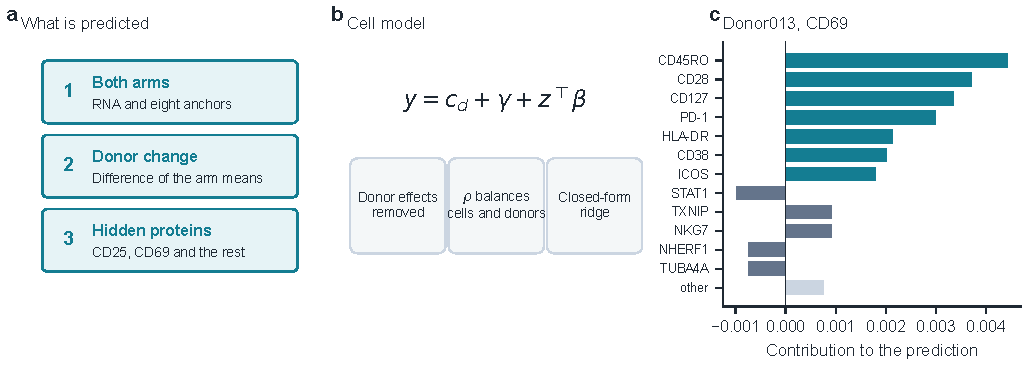
\includegraphics[width=\textwidth]{figures/figure1_model.pdf}
\caption{Task and model. \textbf{(a)} Both arms are observed for RNA and eight anchors. The target is the donor-level change in the hidden proteins. \textbf{(b)} One slope per protein after the donor effects are removed. \textbf{(c)} Largest terms in the exact decomposition of the CD69 prediction for the GSE334503 test donor whose absolute error is closest to the median. Teal bars are anchors. This panel is descriptive and was not used to choose the model.}
\label{fig:model}
\end{figure}

\subsection{Development}
On the nine development tasks, mean standardized MAE across hidden proteins was \DevCb{} for CellBridge, \DevAb{} for abundance shrinkage, \DevJt{} for the joint ridge, \DevRn{} for the RNA ridge and \DevMn{} for the training mean (Figure~\ref{fig:dev}). Forcing anchors into every selected fit, using only single cells, or using only \(\rho=0\) left that mean essentially unchanged (\AblFull{}, \AblAnchor{}, \AblKone{}, \AblRho{}). RNA-only CellBridge rose to \AblRna{}. A greedy panel, adding anchors by inner error, moved the nine-task mean from \PanelZero{} with no anchors to \PanelFour{} with four and \PanelEight{} with eight (Figure~\ref{fig:dev}c). The antibodies chosen differed by task, so the sealed tests kept the prespecified eight. These numbers include previously exposed Lawlor data.

\begin{figure}[t]
\centering
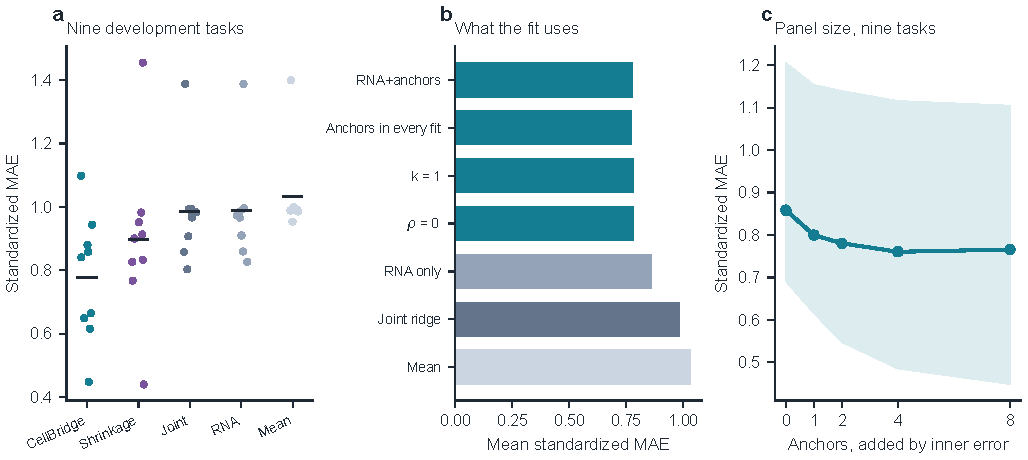
\includegraphics[width=\textwidth]{figures/figure2_development.pdf}
\caption{Development, nine tasks, exploratory. \textbf{(a)} Standardized MAE for all hidden proteins. Bars are means. \textbf{(b)} The full grid against ablations and the pseudobulk baselines. \textbf{(c)} Greedy panel size. The band is the range across tasks.}
\label{fig:dev}
\end{figure}

\subsection{Sealed test: GSE334503}
CellBridge scored \MaeGseCbEone{} on E1 and \MaeGseCbEtwo{} on E2 (Table~\ref{tab:main}, Figure~\ref{fig:gse}). The abundance-shrinkage baseline scored \MaeGseAbEone{} and \MaeGseAbEtwo{}. totalVI scored \MaeGseTvEone{} and \MaeGseTvEtwo{}. The training mean scored \MaeGseMnEone{} and \MaeGseMnEtwo{}.

H1, all hidden proteins against the mean, was rejected: gain \GseHOneGain{} (95\% interval \GseHOneLo{} to \GseHOneHi{}, sign-flip \(p\GseHOneP\), \GseHOneWins{}/\GseHOneN{} donors). H2--H8 were rejected in sequence, including both totalVI comparisons (H7 gain \GseHSevenGain{}, \(p\GseHSevenP\)). H9, all hidden proteins against abundance shrinkage, was not rejected (gain \GseHNineGain{}, interval \GseHNineLo{} to \GseHNineHi{}, \(p\GseHNineP\), \GseHNineWins{}/\GseHNineN{} donors). The sequence stopped there. H10 was recorded and was not tested. The primary claim, H1--H6, was \GseClaim{}. Non-inferiority to abundance shrinkage \GseNiEtwoHold{} on E2 (upper excess \GseNiEtwoUpper{}) and \GseNiEoneHold{} on E1 at the boundary (upper excess \GseNiEoneUpper{}). Conformal coverage on all hidden proteins was \GseCovCb{}, against the nominal level.

The largest individual contributions to one representative CD69 prediction are anchor antibodies (Figure~\ref{fig:model}c). Across proteins, those anchors are a minority of the absolute contribution, because hundreds of genes each add a little (Figure~\ref{fig:panel}b).

\begin{figure}[t]
\centering
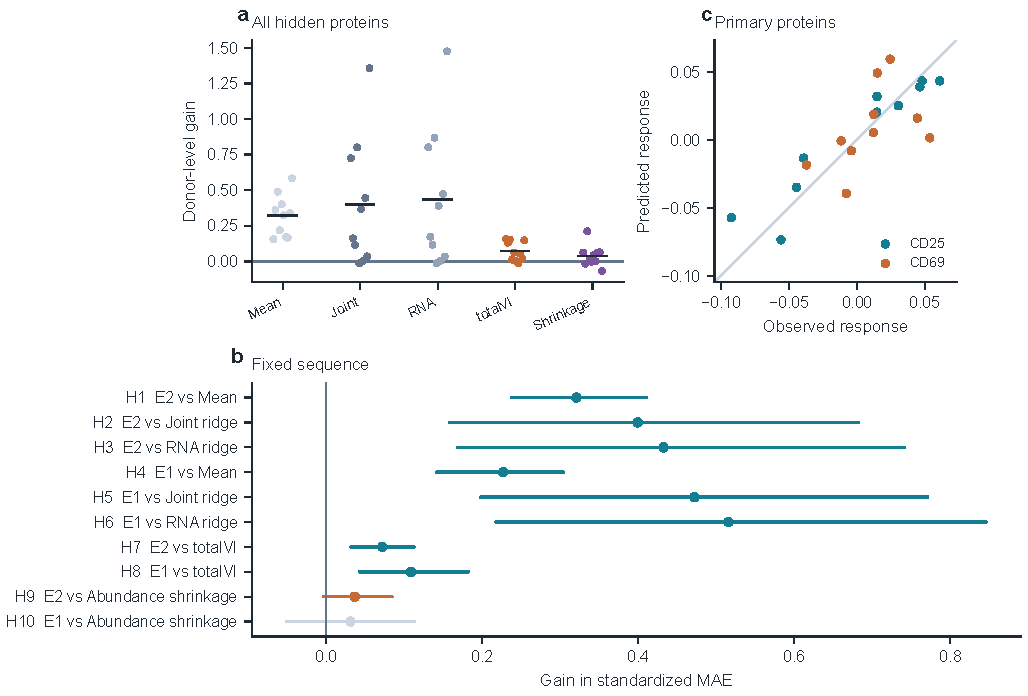
\includegraphics[width=\textwidth]{figures/figure3_gse334503.pdf}
\caption{GSE334503, sealed, \NGseTest{} test donors. \textbf{(a)} Donor-level gain on all hidden proteins. A positive value means CellBridge has lower loss. \textbf{(b)} Fixed sequence. Teal is rejected, orange is tested and not rejected, grey is recorded and not tested. \textbf{(c)} Predicted and observed responses for CD25 and CD69.}
\label{fig:gse}
\end{figure}

\subsection{Replication: E-MTAB-9357}
CellBridge scored \MaeEmCbEone{} on E1 and \MaeEmCbEtwo{} on E2. The abundance-shrinkage baseline scored \MaeEmAbEone{} and \MaeEmAbEtwo{}. totalVI scored \MaeEmTvEone{} and \MaeEmTvEtwo{}, which is worse than the training mean (\MaeEmMnEone{} and \MaeEmMnEtwo{}). Both pseudobulk ridges matched the training mean exactly on this cohort, so H1--H3 are the same comparison three times.

H1 was rejected: gain \EmHOneGain{} (interval \EmHOneLo{} to \EmHOneHi{}, \(p\EmHOneP\), \EmHOneWins{}/\EmHOneN{} donors). H2 and H3 were the same result. H4, CD25 and CD69 against the mean, was not rejected: gain \EmHFourGain{} (interval \EmHFourLo{} to \EmHFourHi{}, \(p\EmHFourP\), \EmHFourWins{}/\EmHFourN{} donors). The sequence stopped at \EmStopped{}. The primary claim was \EmClaim{}. H5--H10 were recorded and were not tested. The recorded totalVI gains are positive, and the recorded gain against abundance shrinkage is about zero (H9 gain \EmHNineGain{}, \(p\EmHNineP\)). Non-inferiority \EmNiEtwoHold{} on E2 (upper excess \EmNiEtwoUpper{}) and \EmNiEoneHold{} on E1 (upper excess \EmNiEoneUpper{}).

RNA-only CellBridge scored \MaeEmRoEtwo{} on E2, close to the mean and far from the full model (Figure~\ref{fig:emtab}d). On this cohort the gain over a pseudobulk RNA model is carried by the eight anchors. Conformal coverage was \EmCovCb{}.

\begin{figure}[t]
\centering
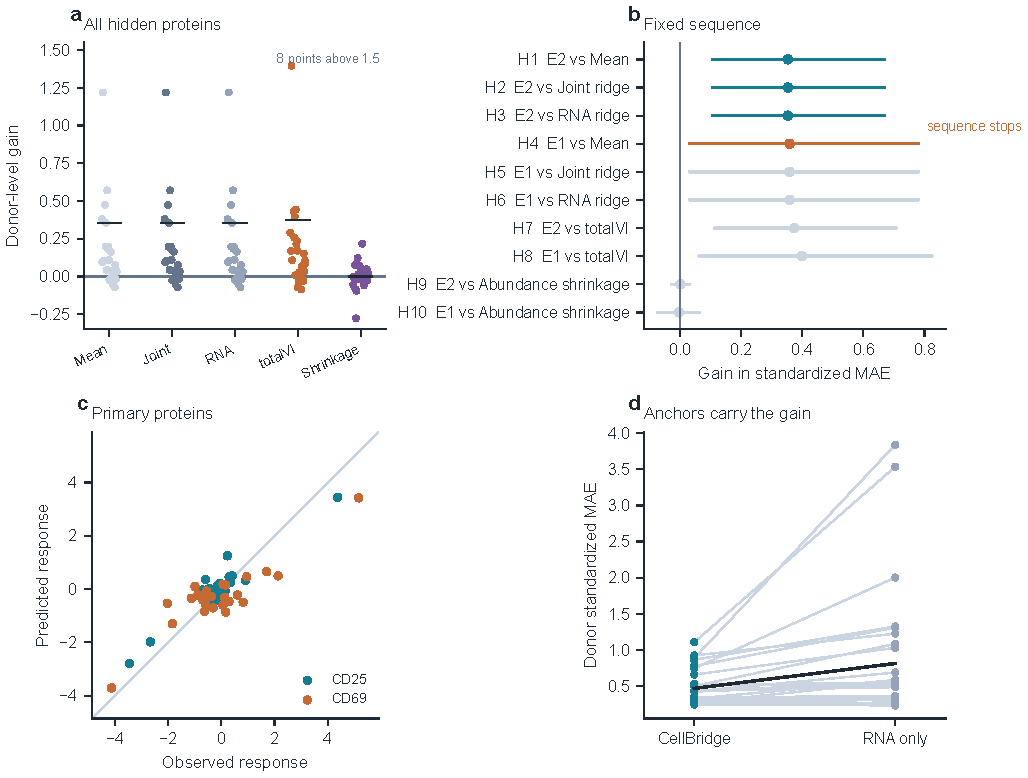
\includegraphics[width=\textwidth]{figures/figure4_emtab9357.pdf}
\caption{E-MTAB-9357, unblinded once, \NEmTest{} test donors. Panels match Figure~\ref{fig:gse}. \textbf{(b)} The sequence stops at H4. Grey intervals were not tested. Donor-level gains above the displayed range in \textbf{(a)} are omitted from the axis and counted in the corner. \textbf{(d)} Each line is one test donor. The black line is the mean.}
\label{fig:emtab}
\end{figure}

\begin{table}[t]
\centering
\caption{Standardized MAE on the sealed tests. Lower is better. E1 is CD25 and CD69. E2 is all hidden proteins. RNA-only CellBridge is descriptive and is not in the sequence.}
\label{tab:main}
\begin{tabular}{@{}lcccc@{}}
\toprule
 & \multicolumn{2}{c}{GSE334503} & \multicolumn{2}{c}{E-MTAB-9357} \\
\cmidrule(lr){2-3}\cmidrule(lr){4-5}
 & E1 & E2 & E1 & E2 \\
\midrule
CellBridge & \MaeGseCbEone & \MaeGseCbEtwo & \MaeEmCbEone & \MaeEmCbEtwo \\
Abundance shrinkage & \MaeGseAbEone & \MaeGseAbEtwo & \MaeEmAbEone & \MaeEmAbEtwo \\
totalVI & \MaeGseTvEone & \MaeGseTvEtwo & \MaeEmTvEone & \MaeEmTvEtwo \\
RNA-only CellBridge & \MaeGseRoEone & \MaeGseRoEtwo & \MaeEmRoEone & \MaeEmRoEtwo \\
Joint ridge & \MaeGseJtEone & \MaeGseJtEtwo & \MaeEmJtEone & \MaeEmJtEtwo \\
RNA ridge & \MaeGseRnEone & \MaeGseRnEtwo & \MaeEmRnEone & \MaeEmRnEtwo \\
Training mean & \MaeGseMnEone & \MaeGseMnEtwo & \MaeEmMnEone & \MaeEmMnEtwo \\
\bottomrule
\end{tabular}
\end{table}

\subsection{Both cohorts, speed and the panel}
The secondary meta-analysis on E2, a positive number meaning CellBridge has lower loss, gives a random-effects gain of \MetaMnRe{} against the mean (SE \MetaMnReSe{}) and \MetaAbRe{} against abundance shrinkage (SE \MetaAbReSe{}). The totalVI random effect is \MetaTvRe{} (SE \MetaTvReSe{}), with visible heterogeneity between the cohorts (Figure~\ref{fig:both}a). Fixed-effect estimates are in the supplement. Conformal coverage stays near the nominal level for CellBridge on both cohorts (Figure~\ref{fig:both}b).

On GSE334503 the CellBridge fit took \GseCbSeconds{} seconds. The totalVI fit took \GseTvSeconds{} seconds (\GseTvMinutes{} minutes) on \GseTvCells{} training cells, plus prediction. On E-MTAB-9357 the totalVI fit took \EmTvSeconds{} seconds. The E-MTAB CellBridge wall time was not stored in the fit receipt, so it is not reported. Building the sufficient statistics for one million cells, eight donors and 30 features took \ScaleMillionSeconds{} seconds in a scaling check (Supplement).

A bootstrap over GSE334503 training donors, on a reduced grid, put an anchor in the largest absolute contribution for \BootCdTwentyFive\% of draws for CD25, \BootCdSixtyNine\% for CD69 and \BootCdOneFiveFour\% for CD154 (Figure~\ref{fig:panel}c). The practical panel result is the development curve: most of the average gain appears by four anchors, and the fifth through eighth do not improve the nine-task mean.

\begin{figure}[t]
\centering
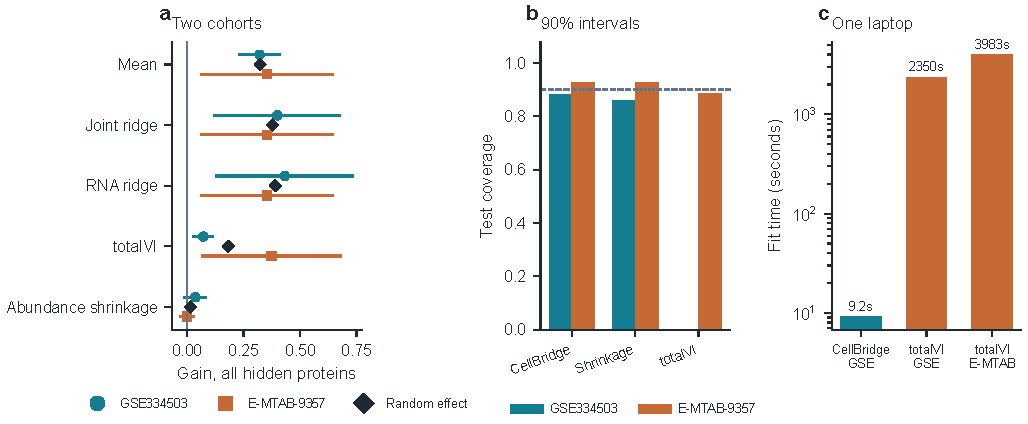
\includegraphics[width=\textwidth]{figures/figure5_synthesis.pdf}
\caption{Both cohorts. \textbf{(a)} Donor-level gains on all hidden proteins, with 95\% intervals, and the random-effects estimate. \textbf{(b)} Split-conformal test coverage at the nominal level. GSE334503 totalVI coverage was not in the sealed conformal record. \textbf{(c)} Fit time on one laptop. The E-MTAB CellBridge time was not in the fit receipt.}
\label{fig:both}
\end{figure}

\begin{figure}[t]
\centering
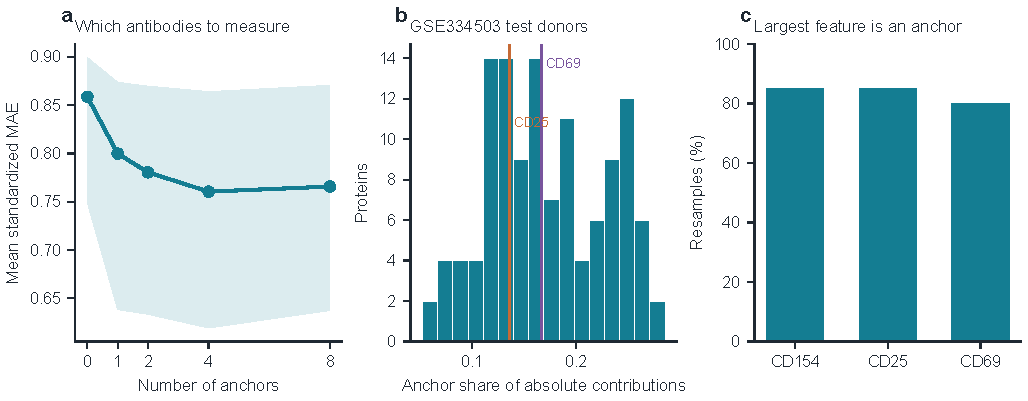
\includegraphics[width=\textwidth]{figures/figure6_panel.pdf}
\caption{What to measure, and what the prediction uses. \textbf{(a)} Greedy panel on the nine development tasks. The band is the interquartile range across tasks. \textbf{(b)} Share of absolute contribution coming from the eight anchors, GSE334503 test donors, one point per protein. \textbf{(c)} Fraction of training-donor bootstrap draws in which the single largest feature is an anchor.}
\label{fig:panel}
\end{figure}

\section{Discussion}
CellBridge is a practical estimator when the target is a donor's protein change and only a few antibodies can be measured. On GSE334503 it beat the training mean, both pseudobulk ridges and one totalVI fit, and it was non-inferior to the strongest donor-level baseline. On E-MTAB-9357 it again beat the mean and the ridges on the all-protein endpoint, the ridges having collapsed to the mean, and it did not clear the primary-endpoint test against the mean. The two cohorts together do not support a claim of superiority over abundance shrinkage. They do support a claim of a fast, closed-form, interpretable model that matches that baseline and is much faster than totalVI.

The E-MTAB result also says where the gain came from. RNA-only CellBridge and both RNA ridges sat on the training mean, while the full model did not. For a follow-up-versus-baseline contrast in hospitalised COVID-19, the eight surface proteins carried the prediction and the transcriptome did not add a detectable donor-level signal under this estimator. That is a limitation of the ``RNA plus a few antibodies'' story, and it is a useful panel result: if the contrast looks like this one, measure the anchors.

Several limits should stay attached to the claims. The Lawlor tasks were used while the method was developed. Both sealed cohorts have tens of test donors, not hundreds, so intervals are wide and H4 on E-MTAB-9357 is a miss by a small margin rather than a precise zero. Feature contributions describe the fitted prediction. They are not causal effects of measuring an antibody. E-MTAB-9357 did not deposit raw UMI counts, and totalVI needed a count scaling and a lower learning rate to train. The totalVI loss on that cohort should be read with those settings. GSE334503's seal time is the laptop clock until the archive is deposited. The E-MTAB-9357 protocol was hashed before unblinding, and the OSF URL was null at the freeze, so this paper does not claim a public preregistration timestamp.

\section*{Data availability}
GSE334503 is available from Zenodo \citep{savi2026}. E-MTAB-9357 is available from ArrayExpress. The sealed predictions, decisions and donor-level losses are in the code repository. The outcome vault used at unblinding is not included.

\section*{Code availability}
CellBridge \texttt{1.0.0} is at \url{https://github.com/armansal1519/cellbridge} under the MIT license. The repository contains the frozen solver, the protocols, the commands that reproduce both cohorts, and the source of this paper.

\section*{Author contributions}
A.S.\ designed the study, wrote the software, ran the sealed evaluations and wrote the manuscript.

\section*{Funding}
None declared.

\section*{Conflict of interest}
None declared.

\bibliographystyle{unsrtnat}
\bibliography{references}
\end{document}
